\thispagestyle{toancuabinone}
\pagestyle{toancuabi}
\everymath{\color{toancuabi}}
\blfootnote{$^*$\color{toancuabi}Nguồn: Câu lạc bộ Toán học Unicorn (UMC)}
\graphicspath{{../toancuabi/pic/}}
\begingroup
\AddToShipoutPicture*{\put(0,616){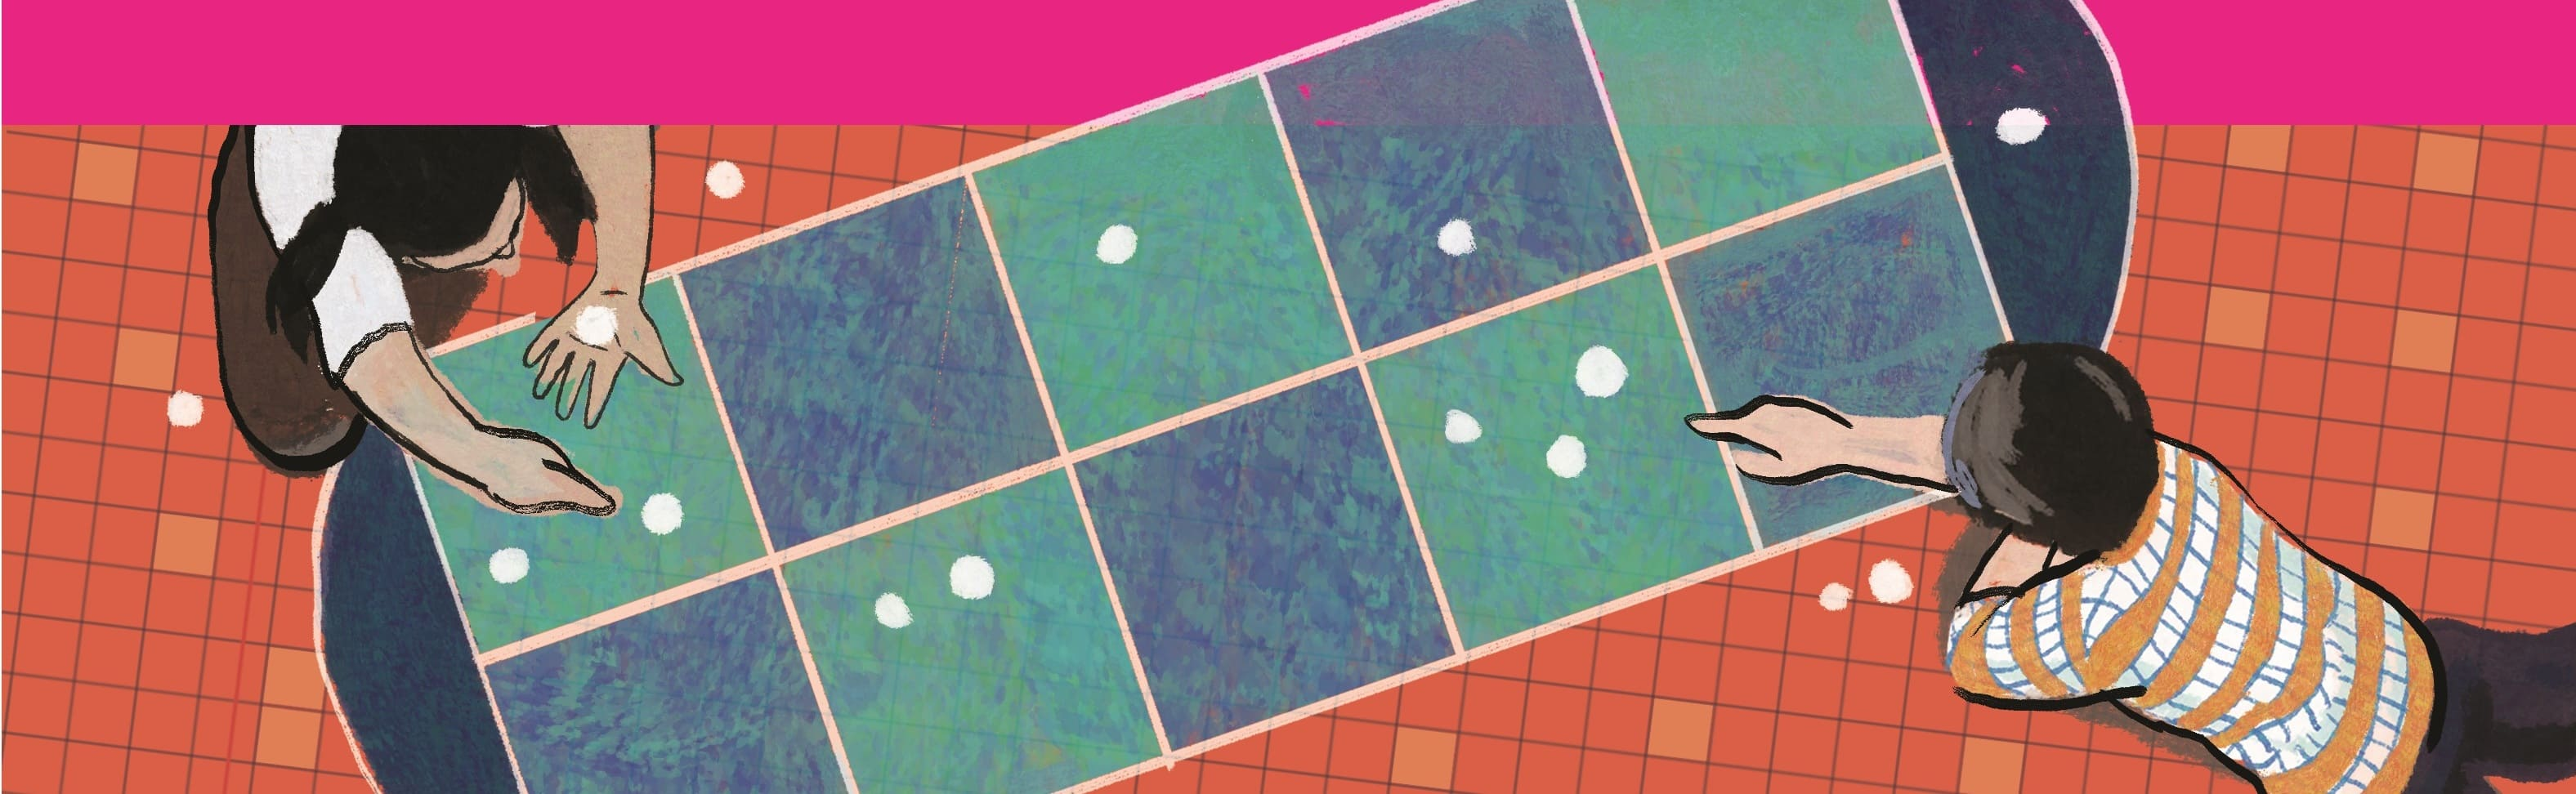
\includegraphics[width=19.3cm]{../bannertoancuabi}}}  
\AddToShipoutPicture*{\put(62,512){
\includegraphics[scale=1]{../tieude1.pdf}}}  
\centering
\endgroup
\vspace*{195pt} 

\definecolor{bulgarianrose}{rgb}{0.28, 0.02, 0.03}
\begin{multicols}{2}
	Trong số này, tạp chí Pi tiếp tục giới thiệu đến với bạn đọc đề thi tuyển sinh năm $2023-2024$ dành cho các bạn học sinh lớp $5$. Các bạn có thể thử sức làm của mình trong khoảng thời gian $90$ phút.
	\vskip 0.1cm
	\textbf{\color{toancuabi}Bài $\pmb1$.} 
	Dựa vào quy luật, hãy cho biết có bao nhiêu dấu thăng trong hình thứ tám của dãy hình sau.
	\begin{figure}[H]
		\vspace*{-5pt}
		\centering
		\captionsetup{labelformat= empty, justification=centering}
		\begin{tikzpicture}[cackithi,scale=0.3,node font=\scriptsize]
			\draw (0,0) grid (2,2);	
			\draw (3,0) grid (7,4);
			\draw (8,0) grid (14,6);
			\draw (15,0) grid (23,8);
			\draw (0.5,0.5) node {$\#$};
			\draw (1.5,0.5) node {$\#$};
			\draw (0.5,1.5) node {$\#$};
			\draw (3.5,0.5) node {$\#$};
			\draw (4.5,0.5) node {$\#$};
			\draw (5.5,0.5) node {$\#$};
			\draw (6.5,0.5) node {$\#$};
			\draw (3.5,1.5) node {$\#$};
			\draw (5.5,1.5) node {$\#$};
			\draw (4.5,2.5) node {$\#$};
			\draw (6.5,2.5) node {$\#$};
			\draw (3.5,3.5) node {$\#$};
			\draw (5.5,3.5) node {$\#$};
			\draw (8.5,0.5) node {$\#$};
			\draw (9.5,0.5) node {$\#$};
			\draw (10.5,0.5) node {$\#$};
			\draw (11.5,0.5) node {$\#$};
			\draw (12.5,0.5) node {$\#$};
			\draw (13.5,0.5) node {$\#$};
			\draw (8.5,1.5) node {$\#$};
			\draw (10.5,1.5) node {$\#$};
			\draw (12.5,1.5) node {$\#$};
			\draw (9.5,2.5) node {$\#$};
			\draw (11.5,2.5) node {$\#$};
			\draw (13.5,2.5) node {$\#$};
			\draw (8.5,3.5) node {$\#$};
			\draw (10.5,3.5) node {$\#$};
			\draw (12.5,3.5) node {$\#$};
			\draw (9.5,4.5) node {$\#$};
			\draw (11.5,4.5) node {$\#$};
			\draw (13.5,4.5) node {$\#$};
			\draw (8.5,5.5) node {$\#$};
			\draw (10.5,5.5) node {$\#$};
			\draw (12.5,5.5) node {$\#$};
			\draw (15.5,0.5) node {$\#$};
			\draw (16.5,0.5) node {$\#$};
			\draw (17.5,0.5) node {$\#$};
			\draw (18.5,0.5) node {$\#$};
			\draw (19.5,0.5) node {$\#$};
			\draw (20.5,0.5) node {$\#$};
			\draw (21.5,0.5) node {$\#$};
			\draw (22.5,0.5) node {$\#$};
			\draw (15.5,0.5) node {$\#$};
			\draw (17.5,0.5) node {$\#$};
			\draw (19.5,0.5) node {$\#$};
			\draw (21.5,0.5) node {$\#$};
			\draw (16.5,1.5) node {$\#$};
			\draw (18.5,1.5) node {$\#$};
			\draw (20.5,1.5) node {$\#$};
			\draw (22.5,1.5) node {$\#$};
			\draw (15.5,2.5) node {$\#$};
			\draw (17.5,2.5) node {$\#$};
			\draw (19.5,2.5) node {$\#$};
			\draw (21.5,2.5) node {$\#$};
			\draw (16.5,3.5) node {$\#$};
			\draw (18.5,3.5) node {$\#$};
			\draw (20.5,3.5) node {$\#$};
			\draw (22.5,3.5) node {$\#$};
			\draw (15.5,4.5) node {$\#$};
			\draw (17.5,4.5) node {$\#$};
			\draw (19.5,4.5) node {$\#$};
			\draw (21.5,4.5) node {$\#$};
			\draw (16.5,5.5) node {$\#$};
			\draw (18.5,5.5) node {$\#$};
			\draw (20.5,5.5) node {$\#$};
			\draw (22.5,5.5) node {$\#$};
			\draw (15.5,6.5) node {$\#$};
			\draw (17.5,6.5) node {$\#$};
			\draw (19.5,6.5) node {$\#$};
			\draw (21.5,6.5) node {$\#$};
			\draw (16.5,7.5) node {$\#$};
			\draw (18.5,7.5) node {$\#$};
			\draw (20.5,7.5) node {$\#$};
			\draw (22.5,7.5) node {$\#$};
			\draw (1,-1) node {Hình $1$};
			\draw (5,-1) node {Hình $2$};
			\draw (11,-1) node {Hình $3$};
			\draw (19,-1) node {Hình $4$};
		\end{tikzpicture}
		\vspace*{-15pt}
	\end{figure}
	\textbf{\color{toancuabi}Bài $\pmb2$.} Bạn Tâm xếp các số $0, 0, 1, 1, 2, 2, 2, 3$ vào các ô vuông trong hình dưới đây (mỗi ô một số) để tạo thành phép trừ của hai số có $4$ chữ số. Hỏi hiệu nhận được lớn nhất có thể là bao nhiêu? 
	\vskip 0.1cm
	Chú ý: \textit{một số có bốn chữ số không được bắt đầu bằng số $0$.}
	\begin{figure}[H]
		\vspace*{-5pt}
		\centering
		\captionsetup{labelformat= empty, justification=centering}
		\begin{tikzpicture}[toancuabi,scale=0.77]
			\draw (0,0) grid (4,1);
			\draw (4.5,0.5) node {$-$};
			\draw (5,0) grid (9,1);
		\end{tikzpicture}
		\vspace*{-10pt}
	\end{figure}
	\textbf{\color{toancuabi}Bài $\pmb3$.} Diện tích của hình được tô đậm bên dưới bằng bao nhiêu?
	\begin{figure}[H]
		\vspace*{5pt}
		\centering
		\captionsetup{labelformat= empty, justification=centering}
		\definecolor{zzttqq}{rgb}{0.6,0.2,0.}
		\begin{tikzpicture}[toancuabi, scale=0.9]
			\fill[color=cackithi,fill=cackithi!40] (1.,0.) -- (2.,5.) -- (3.,0.) -- cycle;
			\fill[color=zzttqq,fill=cackithi!40] (1.,0.) -- (4.,5.) -- (3.,0.) -- (0.,5.) -- cycle;
			\draw  (1.,0.)-- (2.,5.);
			\draw  (2.,5.)-- (3.,0.);
			\draw  (3.,0.)-- (1.,0.);
			\draw  (1.,0.)-- (4.,5.);
			\draw  (4.,5.)-- (3.,0.);
			\draw  (3.,0.)-- (0.,5.);
			\draw  (0.,5.)-- (1.,0.);
			\draw[dashed]  (-1.,5.)-- (5.,5.);
			\draw[dashed]  (-1.,2.5)-- (5.,2.5);
			\draw[dashed]  (-1.,0.)-- (5.,0.);
			\draw[-stealth]  (4.5,5.)-- (4.5,2.5);
			\draw[-stealth]  (4.5,2.5)-- (4.5,0.);
			\draw[-stealth]  (1,-0.4)-- (3.,-0.4);
			
			\draw[-stealth]  (4.5,2.5) -- (4.5,5.);
			\draw[-stealth]  (4.5,0.) -- (4.5,2.5);
			\draw[-stealth]  (3.,-0.4) -- (1,-0.4);
			\draw[color=black] (4.21498164902576,3.87946061896495) node {$5$};
			\draw[color=black] (4.143071467449243,1.3626042637868525) node {$5$};
			\draw[color=black] (2.039698656336115,-0.709930933849792) node {$4$};
		\end{tikzpicture}
		\vspace*{-10pt}
	\end{figure}
	\textbf{\color{toancuabi}Bài $\pmb4$.} Trong bảng ô vuông cỡ $4\times 4$ có điền các số khác $0$ sao cho tích của $4$ số trong mỗi hàng, mỗi cột đều bằng nhau. Cho biết các số trong $9$ ô như hình vẽ, hỏi số ở ô có dấu $*$ bằng bao nhiêu?
	\begin{figure}[H]
		\vspace*{-5pt}
		\centering
		\captionsetup{labelformat= empty, justification=centering}
		\begin{tikzpicture}[toancuabi, node font=\small]
			\draw (0,0) grid (4,4);
			\draw (0.5,0.5) node {$32$};
			\draw (0.5,1.5) node {$4$};
			\draw (0.5,3.5) node {$\dfrac{1}{2}$};
			\draw (1.5,1.5) node {$1$};
			\draw (1.5,2.5) node {$4$};
			\draw (1.5,3.5) node {$32$};
			\draw (2.5,0.5) node {$*$};
			\draw (3.5,0.5) node {$16$};
			\draw (2.5,2.5) node {$8$};
			\draw (3.5,2.5) node {$2$};
		\end{tikzpicture}
		\vspace*{-5pt}
	\end{figure}
	\textbf{\color{toancuabi}Bài $\pmb5$.} Khu vườn của gia đình Tâm được minh họa bằng hình chữ nhật trong hình dưới đây. Biết rằng khu vườn có diện tích $120 \,m^2$ và được chia thành ba luống hình chữ nhật. Phần trồng hoa rộng $2\,m$, diện tích $20 \,m^2$, phần trồng dâu rộng $3\, m$. Hỏi diện tích phần trồng rau là bao nhiêu?
	\begin{figure}[H]
		\vspace*{-5pt}
		\centering
		\captionsetup{labelformat= empty, justification=centering}
		\begin{tikzpicture}[scale=0.4,toancuabi]
			\draw (0,0) rectangle (12,10);
			\draw (2,0) -- (2,10) (2,3) -- (12,3);
			\draw (1,10) node[below] {$2\,m$};
			\draw (1,5) node {Hoa};
			\draw (7,1.5) node {Dâu};
			\draw (7,6.5) node {Rau};
			\draw (12,1.5) node[right] {$3\,m$};
		\end{tikzpicture}
		\vspace*{-5pt}
	\end{figure}
	\textbf{\color{toancuabi}Bài $\pmb6$.} Ba bạn An, Bình, Chi chia đều nhau $30$ chiếc kẹo. An ăn một số chiếc kẹo; Bình ăn một số kẹo bằng với số kẹo mà An còn; Chi ăn số kẹo bằng với tổng số kẹo mà An và Bình đã ăn. Hỏi còn lại bao nhiêu chiếc kẹo?
	\vskip 0.1cm
	\textbf{\color{toancuabi}Bài $\pmb7$.} Một bác nông dân chở một xe ô tô quất cảnh ra chợ Tết để bán. Sau khi bán hết cây quất cuối cùng với giá $230$ nghìn đồng, bác tính nhẩm lại thấy mình đã bán số cây quất với giá trung bình là $245$ nghìn đồng/cây. Nhưng người mua cây quất cuối quay trở lại và chỉ cho bác thấy cành quất bị rụng quá nhiều lá, nên ông ta chỉ đồng ý mua với giá $158$ nghìn đồng. Bác chấp thuận và bán cây quất đó. Khi nhẩm tính lại, bác nông dân thấy giá trung bình của xe quất bây giờ là $242$ nghìn đồng. Hỏi bác đã bán được bao nhiêu cây quất?
	\vskip 0.1cm
	\columnbreak
	\textbf{\color{toancuabi}Bài $\pmb8$.} Có bao nhiêu cách xếp $5$ viên bi giống hệt nhau vào các ô hình vuông ở hình vẽ sau sao cho mỗi ô có không quá $1$ viên bi và không có $2$ viên bi nào trên cùng $1$ hàng hoặc $1$ cột?
	\begin{figure}[H]
		\vspace*{-10pt}
		\centering
		\captionsetup{labelformat= empty, justification=centering}
		\begin{tikzpicture}[toancuabi,scale=0.8]
			\draw  (0.,1.)-- (5.,1.);
			\draw  (5.,1.)-- (5.,4.);
			\draw  (5.,4.)-- (1.,4.);
			\draw  (1.,4.)-- (1.,3.);
			\draw  (1.,3.)-- (0.,3.);
			\draw  (0.,3.)-- (0.,1.);
			\draw  (1.,1.)-- (1.,3.);
			\draw  (1.,2.)-- (5.,2.);
			\draw  (5.,3.)-- (1.,3.);
			\draw  (1.,4.)-- (1.,5.);
			\draw  (1.,5.)-- (2.,5.);
			\draw  (2.,5.)-- (2.,1.);
			\draw  (3.,1.)-- (3.,6.);
			\draw  (3.,6.)-- (4.,6.);
			\draw  (4.,6.)-- (4.,1.);
			\draw  (0.,2.)-- (1.,2.);
			\draw  (3.,5.)-- (4.,5.);
			
			\draw [fill=cackithi!40] (0.,1.) circle (2.0pt);
			\draw [fill=cackithi!40] (5.,1.) circle (2.0pt);
			\draw [fill=cackithi!40] (5.,4.) circle (2.0pt);
			\draw [fill=cackithi!40] (1.,4.) circle (2.0pt);
			\draw [fill=cackithi!40] (1.,3.) circle (2.0pt);
			\draw [fill=cackithi!40] (0.,3.) circle (2.0pt);
			\draw [fill=cackithi!40] (1.,1.) circle (2.0pt);
			\draw [fill=cackithi!40] (1.,2.) circle (2.0pt);
			\draw [fill=cackithi!40] (5.,2.) circle (2.0pt);
			\draw [fill=cackithi!40] (5.,3.) circle (2.0pt);
			\draw [fill=cackithi!40] (1.,5.) circle (2.0pt);
			\draw [fill=cackithi!40] (2.,5.) circle (2.0pt);
			\draw [fill=cackithi!40] (2.,1.) circle (2.0pt);
			\draw [fill=cackithi!40] (3.,1.) circle (2.0pt);
			\draw [fill=cackithi!40] (3.,6.) circle (2.0pt);
			\draw [fill=cackithi!40] (4.,6.) circle (2.0pt);
			\draw [fill=cackithi!40] (4.,1.) circle (2.0pt);
			\draw [fill=cackithi!40] (2.,4.) circle (2.0pt);
			\draw [fill=cackithi!40] (3.,4.) circle (2.0pt);
			\draw [fill=cackithi!40] (4.,4.) circle (2.0pt);
			\draw [fill=cackithi!40] (4.,5.) circle (2.0pt);
			\draw [fill=cackithi!40] (3.,5.) circle (2.0pt);
			\draw [fill=cackithi!40] (4.,3.) circle (2.0pt);
			\draw [fill=cackithi!40] (3.,3.) circle (2.0pt);
			\draw [fill=cackithi!40] (2.,3.) circle (2.0pt);
			\draw [fill=cackithi!40] (2.,2.) circle (2.0pt);
			\draw [fill=cackithi!40] (3.,2.) circle (2.0pt);
			\draw [fill=cackithi!40] (4.,2.) circle (2.0pt);
			\draw [fill=cackithi!40] (0.,2.) circle (2.0pt);
		\end{tikzpicture}
		\vspace*{-5pt}
	\end{figure}
	\textbf{\color{toancuabi}Bài $\pmb9$.} Mỗi ô trong hình bên được điền một số sao cho: số được ghi trong mỗi ô ở $3$ hàng trên cùng bằng tổng $2$ số ở hai ô ngay bên dưới nó. 
	Cho biết trước $3$ số như trong hình vẽ, hỏi số nào phải được điền vào ô có chữ $x$?
	\begin{figure}[H]
		\vspace*{-5pt}
		\centering
		\captionsetup{labelformat= empty, justification=centering}
		\begin{tikzpicture}[xscale=2,scale=0.8,toancuabi]
			\draw (0,0) grid (4,1);
			\draw (1,2) grid (3,3);
			\draw (0.5,1) rectangle (3.5,2);
			\draw (1.5,3) rectangle (2.5,4);
			\draw (1.5,1) --(1.5,2) (2.5,1) --(2.5,2);
			\draw (0.5,0.5) node {$10$};
			\draw (3.5,0.5) node {$12$};
			\draw (2,1.5) node {$x$};
			\draw (2,3.5) node {$100$};
		\end{tikzpicture}
		\vspace*{-5pt}
	\end{figure}
	\textbf{\color{toancuabi}Bài $\pmb{10}$.} Sau khi sạc điện thoại di động, bạn Kiên nhận ra mình đã quên mã PIN (mã gồm $4$ chữ số). Kiên nhớ là mã PIN bắt đầu bằng số $1$, kết thúc bằng số $3$ và các chữ số trong mã đều khác nhau.
	Có bao nhiêu số khác nhau cho mã PIN của Kiên?
	\vskip 0.1cm
	\hfill\textit{Xem lời giải/đáp án trang...} 
\end{multicols}
\newpage
\graphicspath{{../toancuabi/pic/}}
\begingroup
\AddToShipoutPicture*{\put(122,680){
\includegraphics[scale=1]{../tieude.pdf}}}  
\centering
\endgroup
\vspace*{25pt} 
\begin{multicols}{2}
	Thám tử Xuân Phong phải cải trang thành một nhà báo để tìm hiểu về một công ty nước giải khát có uy tín, tuy nhiên mới đây đã bất ngờ bị lộ bí mật về công thức pha chế với đối thủ cạnh tranh. Trong vai trò của một nhà báo, Xuân Phong tham gia một buổi họp đặc biệt gồm $n$ nhân viên chủ chốt của công ty. Xuân Phong được biết rằng, trong số $n$ người này có một người, có bí danh là Z, biết toàn bộ mọi nhân viên còn lại, tuy nhiên không một ai trong số $n-1$ người còn lại lại biết anh ta. Người có bí danh Z này có thể cho Xuân Phong đầu mối vì sao công thức pha chế bị lộ ra ngoài.
	\vskip 0.1cm
	Xuân Phong có thể tới cạnh mỗi một người bất kỳ trong buổi họp, và hỏi anh ta câu hỏi sau: ``Anh có biết <một người nào đó> không?" (trong ngoặc < > là một người cụ thể nào đó trong số những người còn lại). Rất may, khác với mọi lần, lần này  tất cả $n$ người đều nói thật, và Xuân Phong có thể hỏi một người nhiều hơn một lần.
	\vskip 0.1cm
	$a)$ Hỏi Xuân Phong có thể xác định được ai là Z sau khi đưa ra ít hơn $n$ câu hỏi được hay không?
	\vskip 0.1cm
	$b)$ Tìm số câu hỏi ít nhất đủ để Xuân Phong luôn tìm được nhân viên Z. Em hãy chứng minh rằng không thể hỏi ít hơn số câu hỏi như vậy được.
	\begin{figure}[H]
		\centering
		\vspace*{-10pt}
		\captionsetup{labelformat= empty, justification=centering}
		
\includegraphics[width=0.95\linewidth]{xp}
		\vspace*{-5pt}
	\end{figure}
\end{multicols}
\vspace*{-10pt}
{\color{toancuabi}\rule{1\linewidth}{0.1pt}}

\begingroup
\AddToShipoutPicture*{\put(120,295){
\includegraphics[scale=1]{../tieude11.pdf}}} 
\centering
\endgroup
\vspace*{60pt}

\begin{multicols}{2}
	$\pmb{1.}$ Nàng Lọ Lem đi lạc vào trong rừng. Theo lời khuyên của bà tiên, nàng tìm thấy ba chiếc rương đựng những hạt dẻ có thể đem lại điều ước. Chiếc rương thứ nhất có ít hơn $6$ hạt dẻ
	\begin{figure}[H]
		\centering
		\vspace*{-5pt}
		\captionsetup{labelformat= empty, justification=centering}
		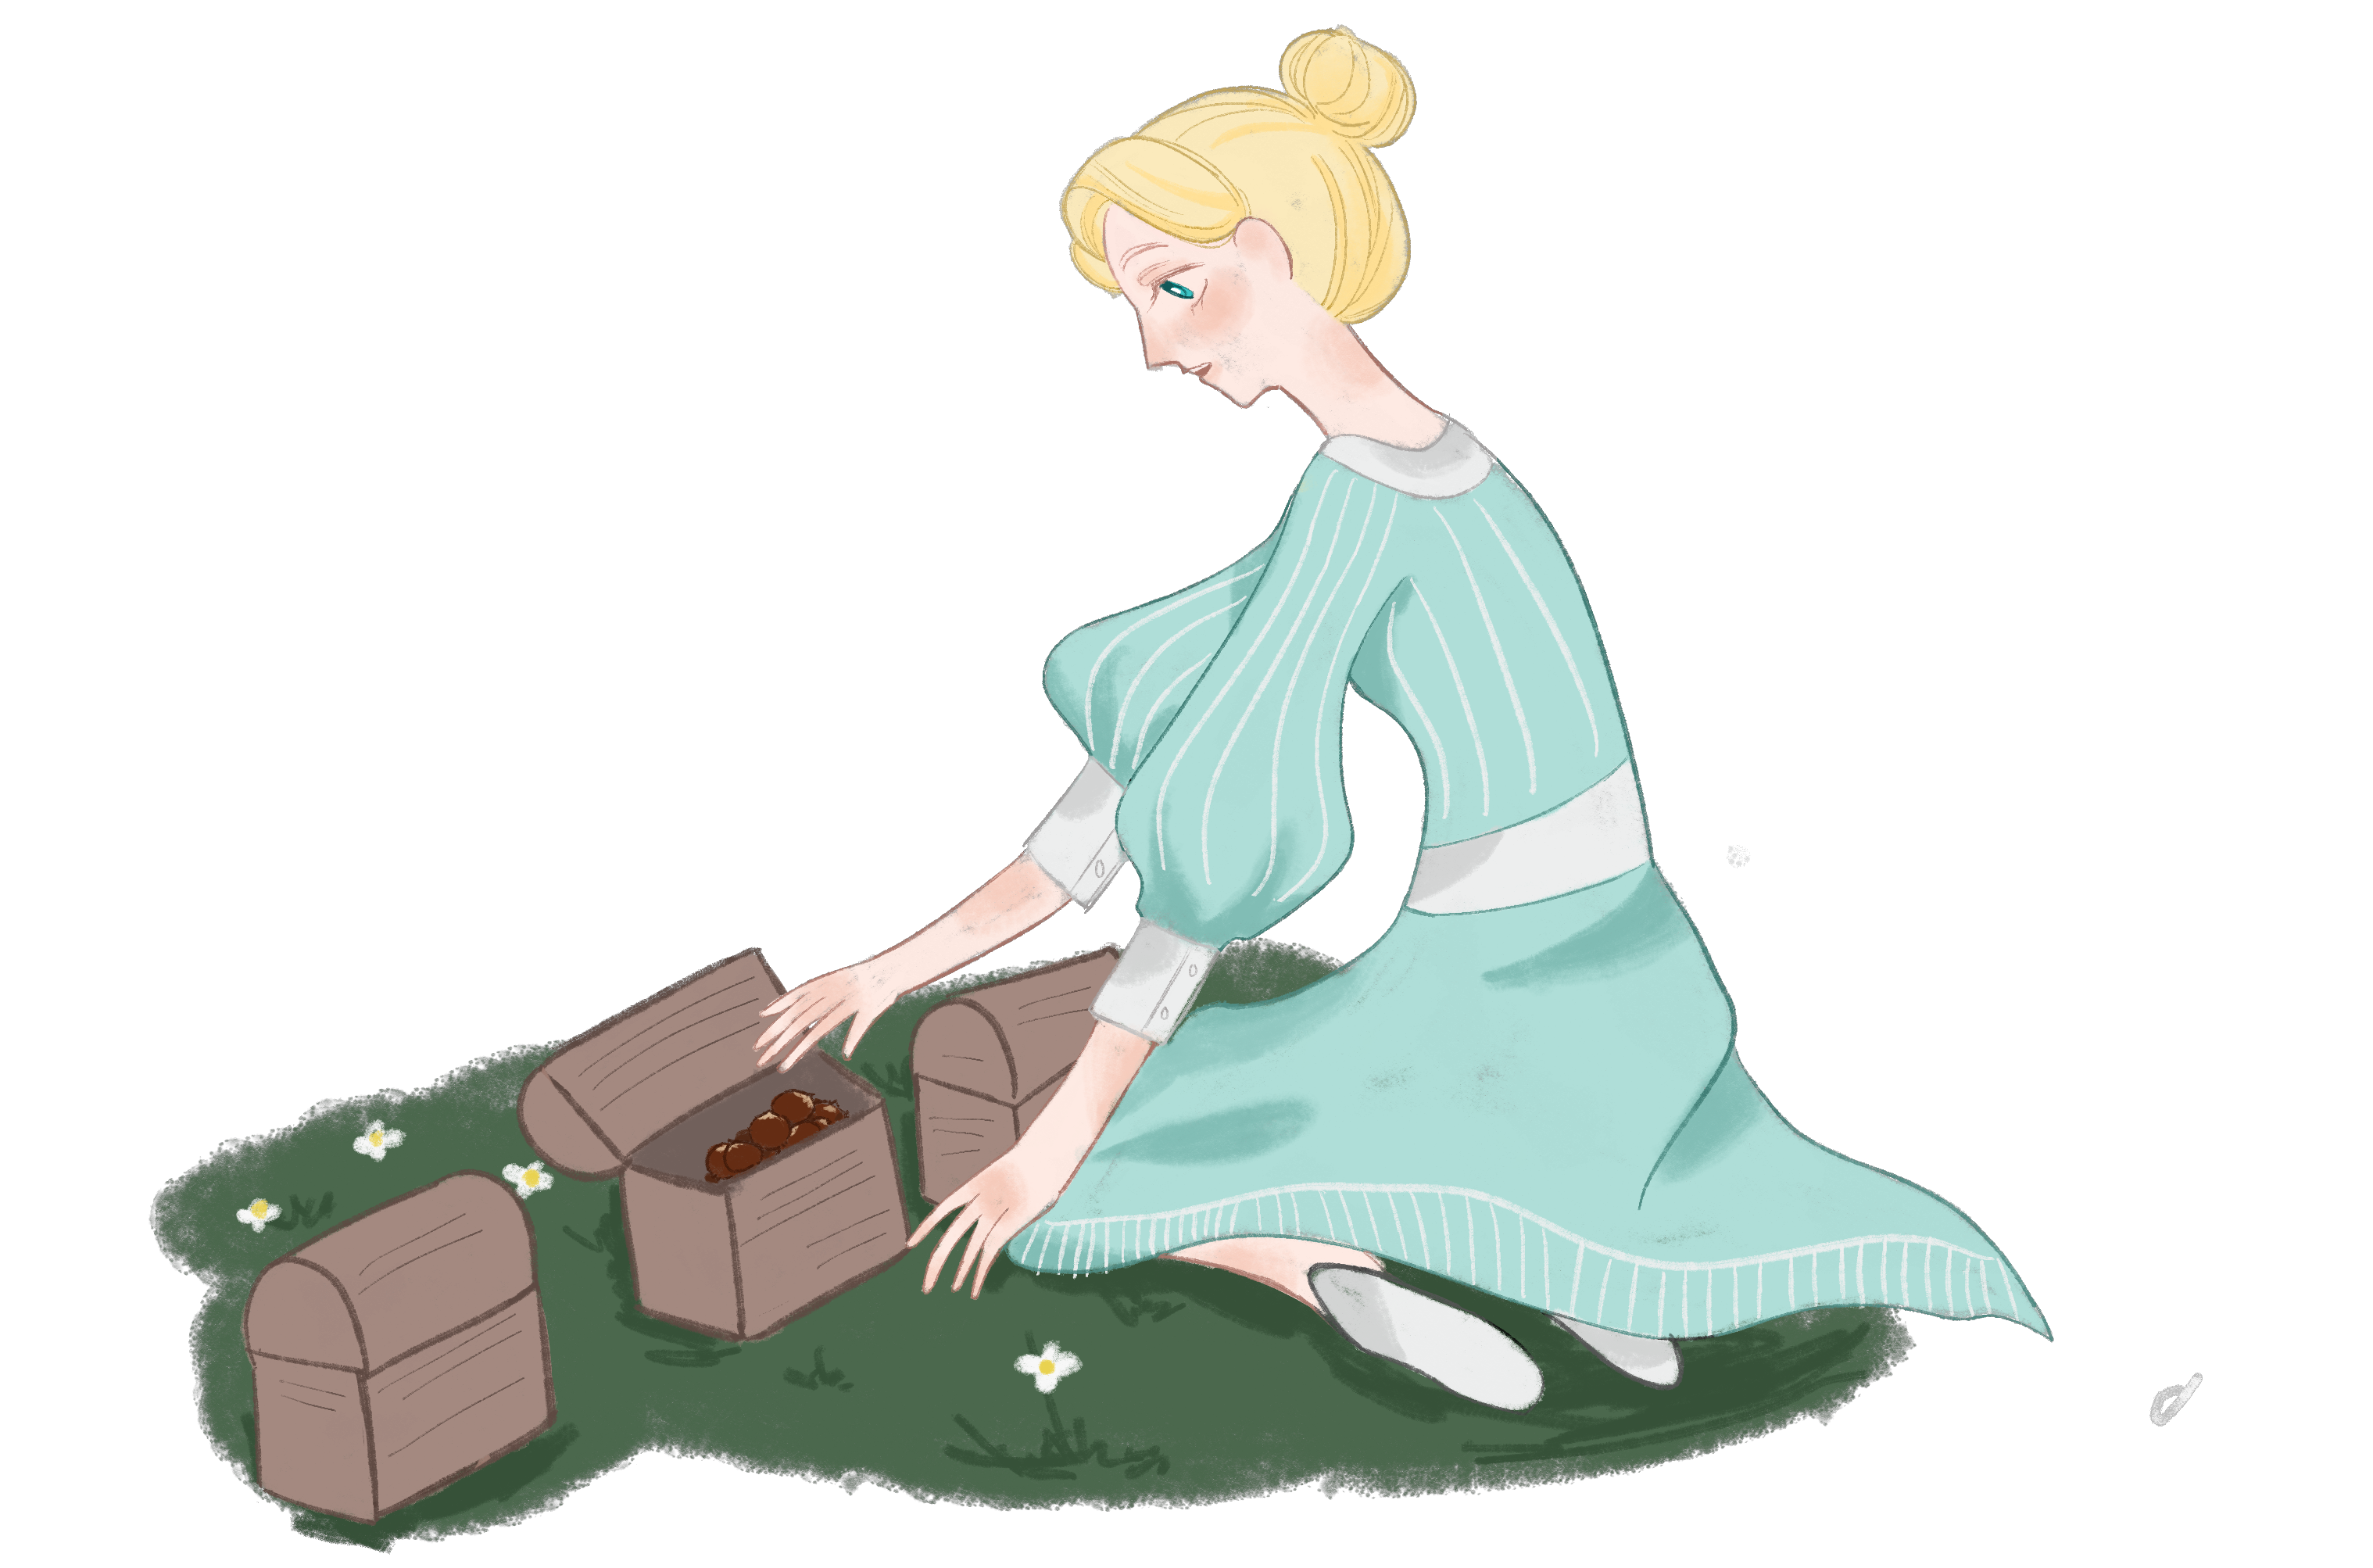
\includegraphics[width=1\linewidth]{Hinh1}
		\vspace*{-5pt}
	\end{figure}
	so với  tổng số hạt dẻ ở hai chiếc rương còn lại. Chiếc rương thứ hai có ít hơn $10$ hạt dẻ so với tổng số hạt dẻ ở chiếc rương thứ nhất và thứ ba. Hỏi trong chiếc rương thứ ba có bao nhiêu hạt dẻ?
	\vskip 0.1cm
	$\pmb{2.}$ Bạn Vân viết $150$ chữ số xung quanh một vòng tròn. Nếu đọc $150$ chữ số này theo chiều kim đồng hồ bắt đầu từ một chỗ nào đó bất kì, thì Vân thấy số nhận được chia hết cho $27$. Em hãy chứng minh rằng, nếu Vân bắt đầu từ bất kỳ một chỗ khác và đọc ngược chiều kim đồng hồ toàn bộ $150$ chữ số đã viết, thì bạn cũng nhận được một số chia hết cho $27$.
	\begin{figure}[H]
		\centering
%		\vspace*{-5pt}
		\captionsetup{labelformat= empty, justification=centering}
		
\includegraphics[width=0.85\linewidth]{Hinh2}
		\vspace*{-5pt}
	\end{figure}
	$\pmb{3.}$ Có ba tên cướp ăn trộm được $10$ viên kim cương trong một két sắt với tổng giá trị là $4 000 000$ dollar. Chúng dự định sẽ phân chia những viên kim cương này cho nhau để mỗi tên có được ít nhất $1 000 000$ dollar. Khi bị cảnh sát truy đuổi, một viên kim cương trị giá $600 000$ dollar bị rơi mất, và vì thế chúng không thể chia được những viên kim cương như dự định ban đầu. Hỏi ba tên cướp này có bị nhầm lẫn ở đâu không, hay là trước khi bị rơi viên kim cương, việc chia đồ ăn trộm của chúng đã không thể thực hiện được theo như dự định?
	\begin{figure}[H]
		\centering
		\vspace*{-5pt}
		\captionsetup{labelformat= empty, justification=centering}
		
\includegraphics[width=1\linewidth]{Hinh3}
		\vspace*{-15pt}
	\end{figure}
	$\pmb{4.}$ 	Bác Tâm mua một bao tải gạo nặng $9$ kg. Bác muốn chia ra thành hai túi nhỏ hơn, một túi nặng $2$ kg, còn túi kia nặng $7$ kg. Bác chỉ có một bàn cân đĩa thăng bằng với hai quả cân, một quả nặng $50$ g, còn quả kia nặng $200$ g. Em hãy giúp bác Tâm thực hiện phép san gạo ra hai túi nhỏ như trên chỉ tối đa sau ba lần cân.
	\begin{figure}[H]
		\centering
		%		\vspace*{-5pt}
		\captionsetup{labelformat= empty, justification=centering}
		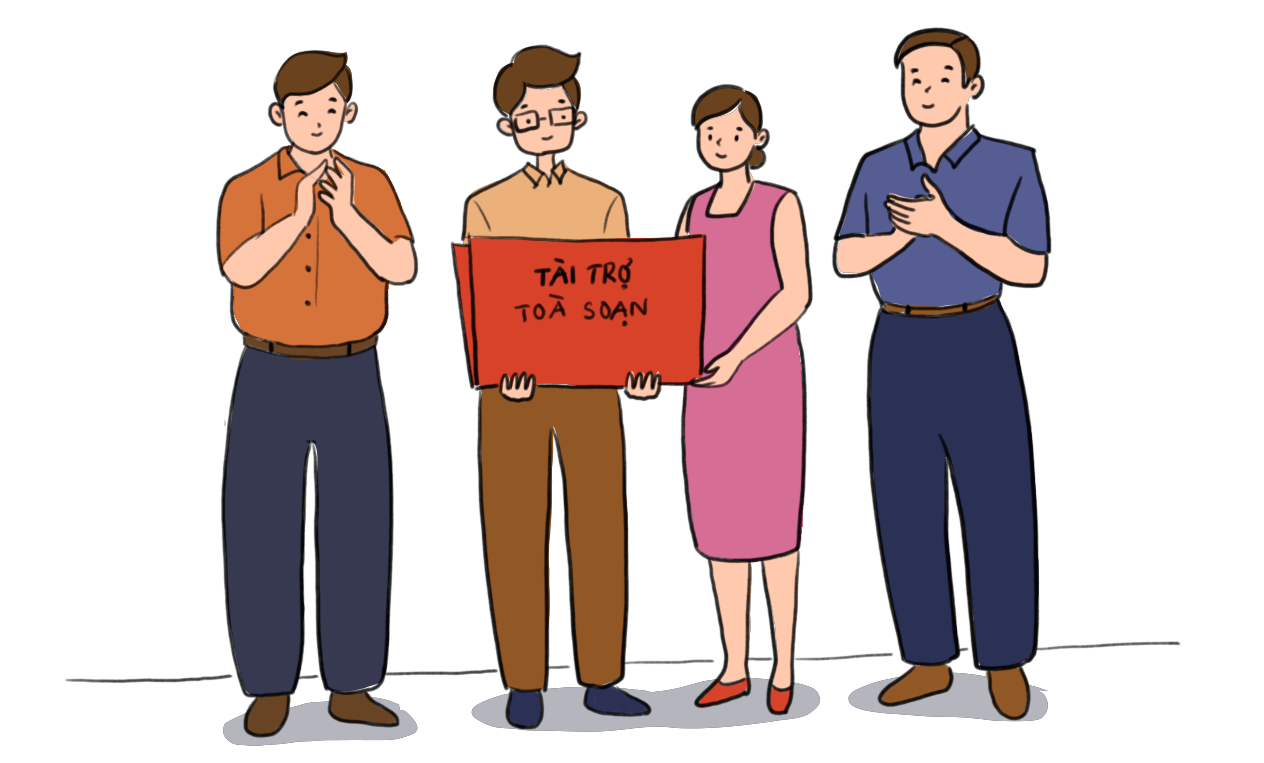
\includegraphics[width=1\linewidth]{Hinh4}
		\vspace*{-10pt}
	\end{figure}
	\vskip 0.1cm
	$\pmb{5.}$ 	Có $6$ đồng xu hình thức bên ngoài giống hệt nhau. Bốn đồng xu trong số đó là thật, mỗi đồng có khối lượng đúng $4$ g, còn hai đồng xu là giả có tổng khối lượng là $8$ g nhưng có một đồng nặng hơn một chút, còn một đồng nhẹ hơn một chút. Hỏi có thể sử dụng một bàn cân thăng bằng (không có quả cân) để sau tối đa bốn lần cân phát hiện được hai đồng xu giả được hay không?
	\begin{figure}[H]
		\centering
		\vspace*{-5pt}
		\captionsetup{labelformat= empty, justification=centering}
		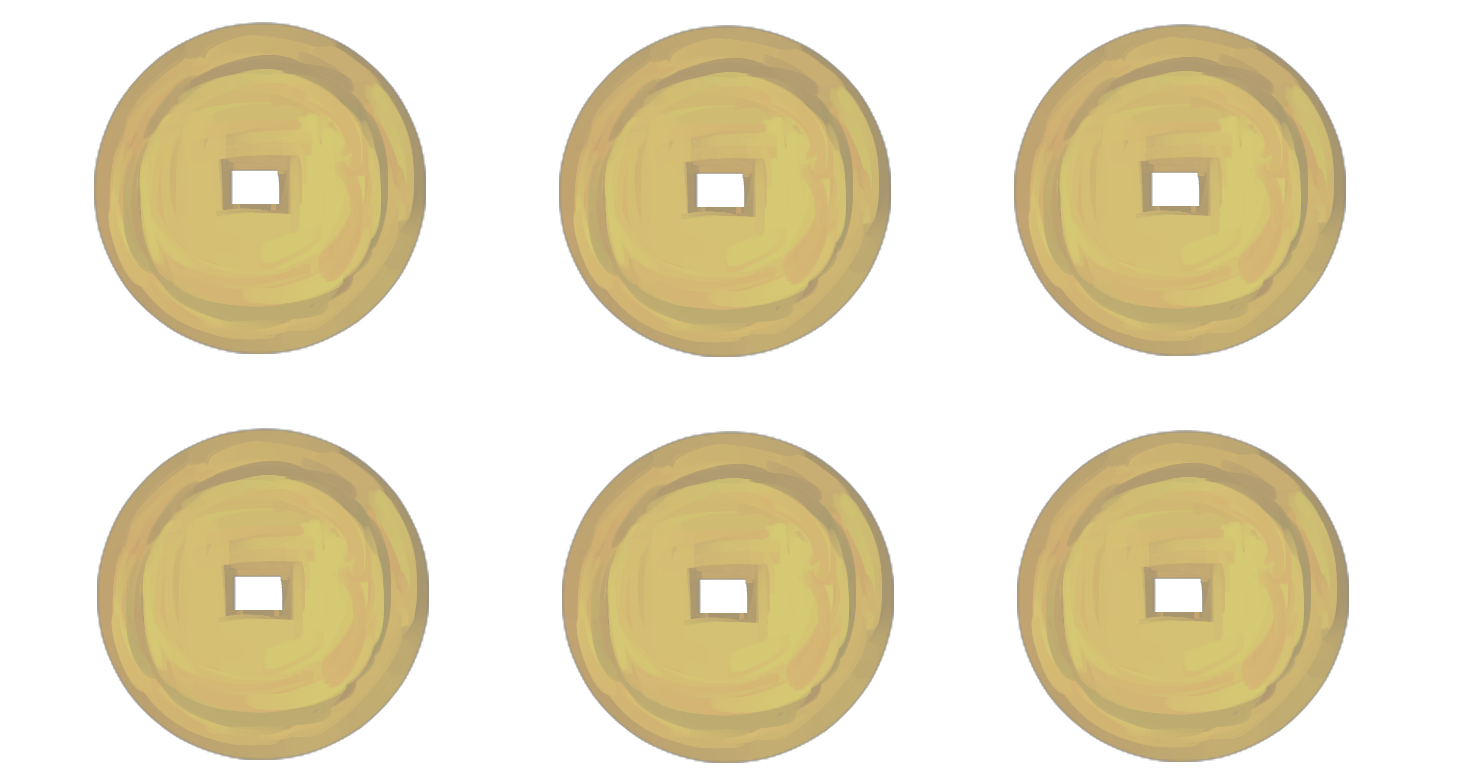
\includegraphics[width=1\linewidth]{Hinh5}
		\vspace*{-20pt}
	\end{figure}
	$\pmb{6.}$ 	Trong một giải vô địch đá bóng của trường, đội dành huy chương vàng có được tổng số điểm là $7$, đội dành huy chương bạc có tổng số điểm là $5$, còn đội dành huy chương đồng có tổng số điểm là $3$. Biết rằng trong giải đấu này các đội thi đấu theo hình thức vòng tròn $1$ lượt, mỗi đội thi đấu với một đội khác đúng một trận, và trong mỗi trận mỗi đội sẽ nhận được $2$ điểm nếu thắng, $1$ điểm nếu hoà, $0$ điểm nếu thua. Nếu hai đội có cùng tổng số điểm thì vị trí thứ tự sẽ được xác định bằng hiệu số bàn thắng và bàn thua. Hỏi 
	\vskip 0.1cm
	$a)$ Đội đứng ở vị trí thấp nhất có được tổng số điểm là bao nhiêu?
	\vskip 0.1cm
	$b)$	Có bao nhiêu đội tham gia giải vô địch.
	\begin{figure}[H]
		\centering
		\vspace*{-10pt}
		\captionsetup{labelformat= empty, justification=centering}
		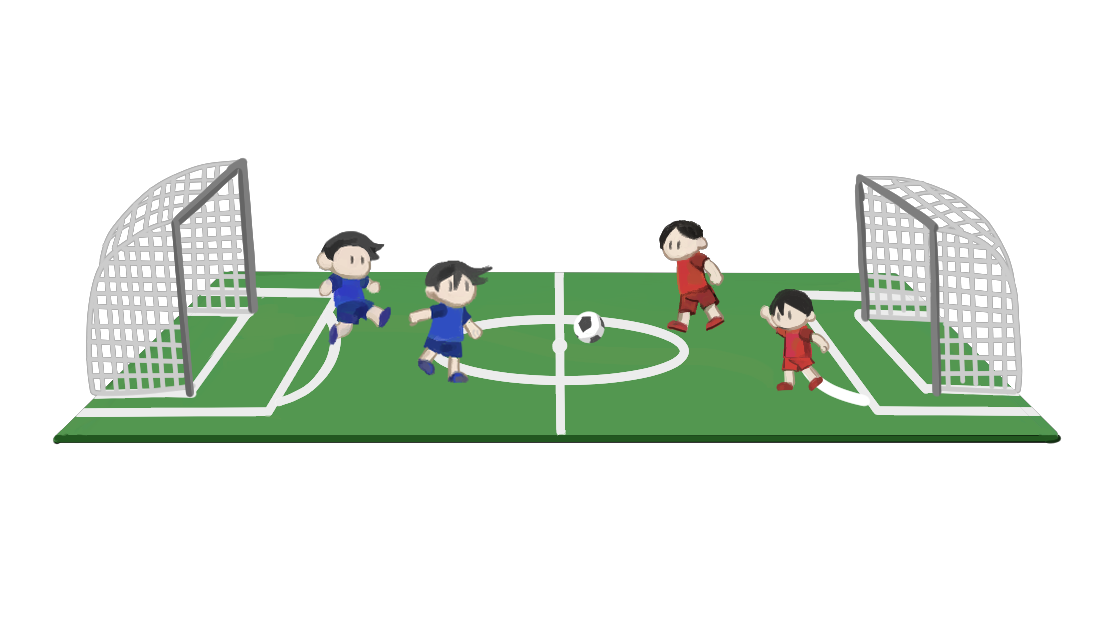
\includegraphics[width=1\linewidth]{Hinh6}
		\vspace*{-10pt}
	\end{figure}
\end{multicols}
\newpage
\begingroup
\AddToShipoutPicture*{\put(116,640){
\includegraphics[scale=1]{../tieude2.pdf}}} 
\centering
\endgroup
\vspace*{65pt}

\begin{multicols}{2}
	$\pmb{1.}$ 	Tại thành phố Hoa Hướng Dương, trong số các cậu bé tí hon có $5$ cậu ngày nào cũng ăn bánh rán ngọt, có $7$ cậu bé cứ cách một ngày lại ăn bánh rán ngọt, còn tất cả các cậu bé tí hon còn lại không bao giờ ăn bánh rán ngọt. Ngày hôm qua có $9$ cậu bé tí hon đã ăn bánh rán ngọt. Hỏi trong ngày hôm nay sẽ có bao nhiêu cậu bé tí hon ăn bánh rán ngọt?
	\begin{figure}[H]
		\centering
		\vspace*{-10pt}
		\captionsetup{labelformat= empty, justification=centering}
		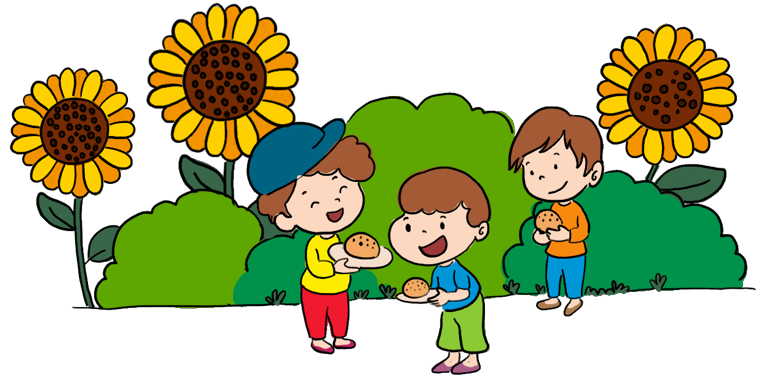
\includegraphics[width=0.9\linewidth]{Pi9_bai1}
		\vspace*{-15pt}
	\end{figure}
	\textit{Lời giải.} 	Trong số $9$ cậu bé tí hon ăn bánh rán ngọt ngày hôm qua có $5$ cậu ăn bánh rán mỗi ngày, như vậy $4$ cậu còn lại ăn bánh rán cách $1$ ngày. Do đó trong ngày hôm nay $4$ cậu này sẽ không ăn bánh rán, còn những cậu bé còn lại (có $3$ cậu) trong số các cậu ăn bánh cách $1$ ngày lại sẽ ăn bánh. Vì thế $3$ cậu này sẽ ăn bánh trong ngày hôm nay, cùng với cả $5$ cậu ăn bánh rán mỗi ngày. Ta có đáp số là: $3+5 = 8$ (cậu bé tí hon).
	\vskip 0.1cm
	$\pmb{2.}$ Một cửa hàng bán hoa tươi có ba loại hoa hồng: hồng tím, hồng vàng và hồng đỏ. Số hoa hồng tím bằng một nửa tổng số hoa hồng vàng và hồng đỏ. Số hoa hồng đỏ lại bằng một phần ba tổng số hoa hồng vàng và số hoa hồng tím. Biết rằng số hoa hồng vàng là $45$ bông. Hỏi cửa hàng có bao nhiêu hoa hồng tím và hoa hồng đỏ?
	\vskip 0.1cm
	\textit{Lời giải.} 	Số hoa hồng tím bằng một nửa tổng số hoa hồng vàng và hồng đỏ, có nghĩa là số hoa hồng tím bằng $1/3$ tổng số hoa hồng. Tương tự, số hoa hồng đỏ chiếm $1/4$ tổng số hoa hồng. Ta có thể vẽ sơ đồ đoạn thẳng, có độ dài bằng $12$ đoạn nhỏ (cho thuận tiện việc biểu diễn $1/3$ và $1/4$ tổng số). Số hoa hồng tím tương ứng $4$ đoạn nhỏ, còn số hoa hồng đỏ tương ứng $3$ đoạn. Suy ra số hoa hồng vàng tương ứng với $12 - 3 - 4 = 5$ (đoạn). Như vậy mỗi đoạn nhỏ tương ứng với $45/5 = 9$ (bông hoa). Do đó, số hoa hồng tím là $4\times 9=36$ (bông) và số hoa hồng đỏ là $3\times 9=27$ (bông).
	\begin{figure}[H]
		\centering
		\vspace*{-10pt}
		\captionsetup{labelformat= empty, justification=centering}
		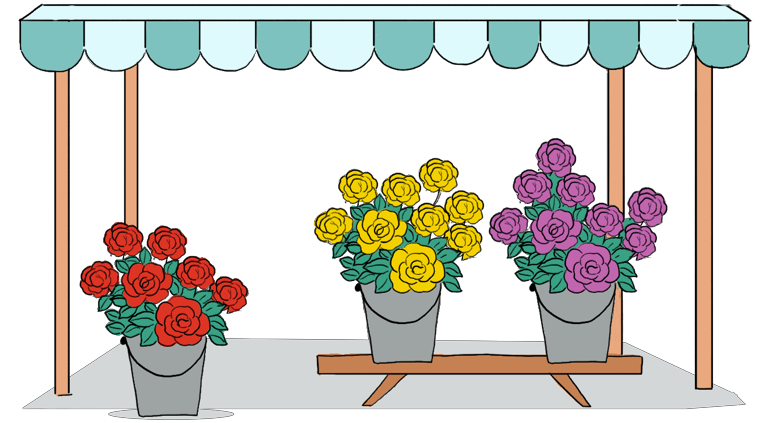
\includegraphics[width=0.8\linewidth]{Pi9_bai2}
		\vspace*{-10pt}
	\end{figure}
	$\pmb{3.}$ Thỏ Hồng đi đón $3$ cậu bạn của mình là Ngựa Đốm, Ngựa Bạch và Gấu Nâu lặn lội đến thăm nhà mình. Vừa ra tới bìa rừng, Thỏ Hồng đã thấy lờ mờ ba bạn đứng hàng ngang ở xa xa ngoài bãi cỏ, nhưng vì sương mù dày đặc, Thỏ Hồng không thể nhận ra ai với ai. Thỏ Hồng bèn kêu các bạn tự giới thiệu để biết được từng vị khách. Cậu bạn đứng ở ngoài cùng bên trái từ vị trí quan sát của Thỏ Hồng nói rằng: ``Có Gấu Nâu đứng cạnh tôi đấy". Cậu bạn đứng ở ngoài cùng bên tay phải, lại tuyên bố rằng: ``Đó là Ngựa Bạch vừa nói với cậu đấy". Cuối cùng, cậu bạn đứng ở giữa, thông báo rằng: ``Bên tay trái của tôi là Ngựa Đốm đấy". Các em hãy tìm ra bạn nào đứng ở đâu trong số $3$ người bạn của Thỏ Hồng, biết rằng Ngựa Đốm thì chuyên nói dối, Ngựa Bạch thì thỉnh thoảng nói dối, còn Gấu Nâu thì không bao giờ nói dối Thỏ Hồng.
	\vskip 0.1cm
	\textit{Lời giải.} Nếu như Gấu Nâu đứng ở ngoài cùng bên trái (từ vị trí quan sát của Thỏ Hồng), thì cậu bạn đứng giữa cũng phải là Gấu Nâu -- điều này là mâu thuẫn. Nếu như Gấu Nâu đứng ở giữa, thì bên tay phải (theo Thỏ Hồng quan sát) sẽ là Ngựa Đốm, còn bên ngoài cùng tay trái sẽ là Ngựa Bạch. Nhưng như vậy, Ngựa Đốm sẽ nói thật, ta lại suy ra mâu thuẫn.
	\begin{figure}[H]
		\centering
		\vspace*{-10pt}
		\captionsetup{labelformat= empty, justification=centering}
		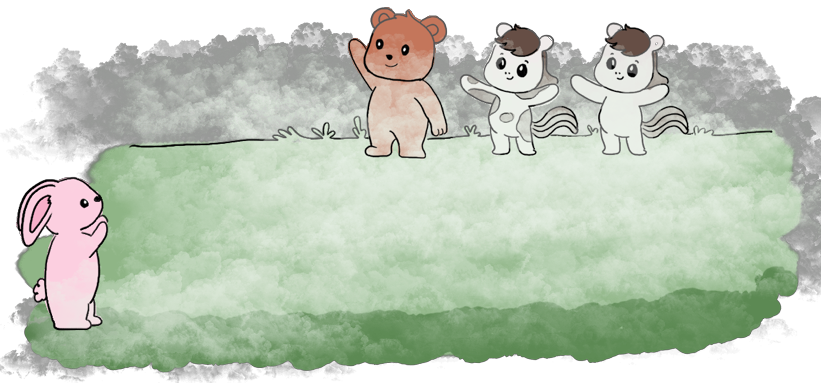
\includegraphics[width=0.85\linewidth]{Pi9_bai3}
		\vspace*{-10pt}
	\end{figure}
	Cuối cùng, chỉ khi Gấu Nâu đứng ngoài cùng bên phải ta mới không gặp mâu thuẫn. Khi đó ngoài cùng tay trái là Ngựa Bạch, ở giữa là là Ngựa Đốm -- hai cậu bạn này đều nói dối.
	\vskip 0.1cm
	\textit{Đáp số}: Từ chỗ quan sát của Thỏ Hồng, ngoài cùng tay trái là Ngựa Bạch, ở giữa là Ngựa Đốm, còn đứng ngoài cùng bên phải là Gấu Nâu.
	\vskip 0.1cm
	$\pmb{4.}$ Có $7$ quả táo, khối lượng mỗi quả có thể khác nhau để ở trên bàn. Bạn Thanh nhận thấy rằng có thể đặt $3$ quả trên một đĩa cân và $4$ quả còn lại trên đĩa cân bên kia sao cho hai bên cân thăng bằng. Bạn Thịnh lại thấy rằng có thể đặt $2$ quả táo trên một đĩa cân, và $5$ quả còn lại trên đĩa cân bên kia và hai bên cân cũng thăng bằng. Em hãy chỉ ra rằng có thể đặt trên một đĩa cân bên này $1$ quả táo và đặt trên đĩa cân bên kia $3$ quả táo trong số $7$ quả đã cho, sao cho hai bên cân cũng vẫn thăng bằng.
	\begin{figure}[H]
		\centering
		\vspace*{-10pt}
		\captionsetup{labelformat= empty, justification=centering}
		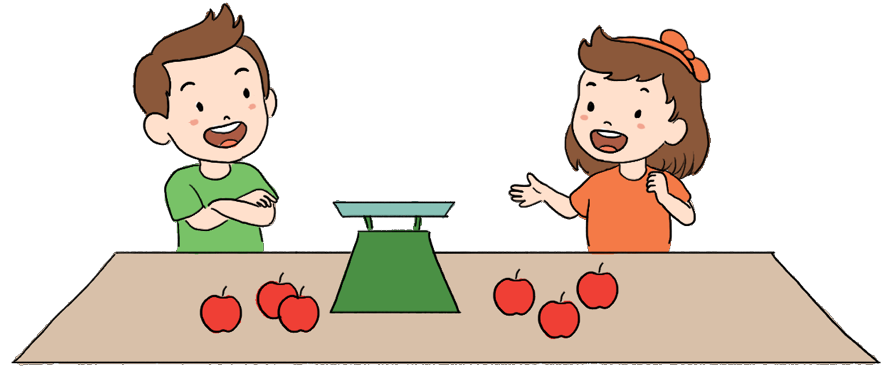
\includegraphics[width=0.85\linewidth]{Pi9_bai4}
		\vspace*{-10pt}
	\end{figure}
	\textit{Lời giải.} 	Để dễ dàng hình dung, ta có thể giả sử rằng Thanh đặt được $3$ quả táo đỏ ở đĩa cân bên trái và $4$ quả táo xanh ở đĩa cân bên phải để cân thăng bằng. Vì vậy nếu Thịnh đặt bất kỳ hai quả táo cùng màu ở một bên và $5$ quả còn lại ở đĩa bên kia thì $5$ quả này sẽ luôn nặng hơn (điều này cũng tương đương với việc có những quả táo nào đó sau lần cân thăng bằng của Thanh đã bị chuyển sang đĩa cân bên kia).
	\vskip 0.1cm
	Vì vậy để cho cân thăng bằng, Thịnh chỉ có thể đặt hai quả táo khác màu trên một đĩa cân, và $5$ quả còn lại sang đĩa bên kia. Nhưng điều này cũng tương đương với việc sau khi Thanh đã cân được thăng bằng, Thịnh đã đổi chỗ $2$ quả táo đỏ với $1$ quả táo xanh. Nếu như bỏ $3$ quả này đi, thì trên một đĩa cân có $1$ quả táo đỏ và trên đĩa bên kia có $3$ quả táo xanh, và hơn nữa cân hai bên vẫn thăng bằng.
	\vskip 0.1cm
	Các em có thể làm bài này bằng lập luận theo dạng của biểu thức đại số, lập ra hai phương trình và tìm hiệu của chúng.
	\vskip 0.1cm
	$\pmb{5.}$ Có $20$ chiếc túi nilon, mỗi túi đựng $26$ quả mận. Biết rằng tổng khối lượng của mỗi túi không vượt quá $1$ kg. Em hãy chỉ ra rằng có thể xếp số mận trên vào $26$ chiếc túi nilon, mỗi túi có đúng $20$ quả mận, sao cho tổng khối lượng của mỗi túi nhỏ hơn $1$ kg.
	\begin{figure}[H]
		\centering
		\vspace*{-10pt}
		\captionsetup{labelformat= empty, justification=centering}
		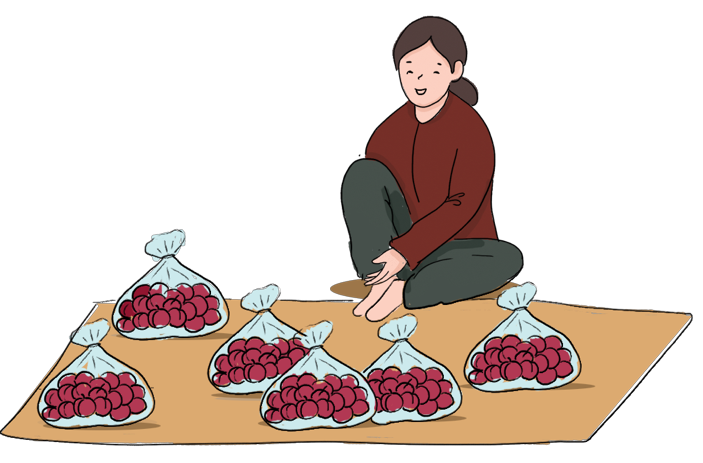
\includegraphics[width=0.85\linewidth]{Pi9_bai5}
		\vspace*{-10pt}
	\end{figure}
	\textit{Lời giải.} 	Ta nhặt ra từ mỗi túi ban đầu quả mận nhẹ nhất và xếp chúng vào chiếc túi thứ $21$. Do mỗi quả nhẹ nhất này có khối lượng không quá $\dfrac{1}{26}$ kg, nên tổng khối lượng của $20$ quả được nhặt ra này không quá $\dfrac{20}{26} <1$ (kg). Hơn nữa khối lượng của mỗi túi ban đầu giờ đều nhẹ hơn $1$ kg, và trong mỗi túi có đúng $25$ quả. Ta lại lặp lại quá trình trên: nhặt ra trong mỗi túi trong số $20$ túi ban đầu quả mận nhẹ nhất (tức là quả mận nhẹ thứ nhì, sau khi đã nhặt ra lần đầu tiên), và đưa $20$ quả này vào chiếc túi thứ $22$, khi đó tổng khối lượng mận ở chiếc túi thứ $22$ này sẽ nhỏ hơn $\dfrac{20}{25}$ (kg). Ta cứ làm như vậy, cho đến khi đạt đến chiếc túi thứ $26$ (sau $6$ lần nhặt ra).
	\vskip 0.1cm
	$\pmb{6.}$ 	Có $100$ số $1, 2, 3, \ldots, 100$ được viết ra thành hàng ngang từ trái qua phải theo thứ tự tăng dần. Bạn Long và bạn Lâm chơi một trò chơi như sau. Hai bạn lần lượt đến lượt chơi của mình sẽ đặt duy nhất một trong các dấu $+$, $-$ hoặc $\times$ vào vị trí bất kỳ xen kẽ giữa hai số trong $100$ số nói trên. Bạn đi lượt cuối cùng sẽ thắng nếu số nhận được bằng cách 
	\begin{figure}[H]
		\centering
		\vspace*{-5pt}
		\captionsetup{labelformat= empty, justification=centering}
		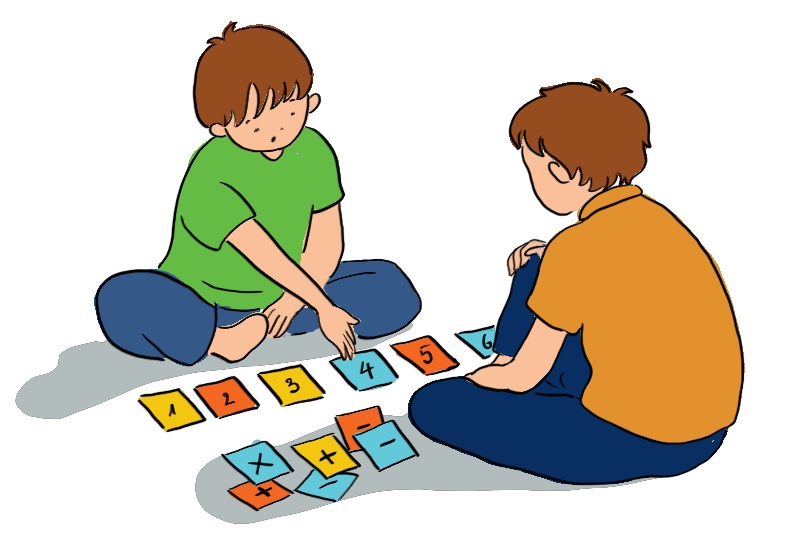
\includegraphics[width=0.7\linewidth]{Pi9_bai6}
		\vspace*{-5pt}
	\end{figure}
	 thực hiện phép tính bởi $100$ số và các phép tính đã điền giữa chúng là một số lẻ. Em hãy chỉ ra rằng nếu Long là người đi đầu tiên (và cũng sẽ là người đi cuối cùng) thì Long luôn có cách chơi để thắng.
	\vskip 0.1cm
	\textit{Lời giải.} 	Trước tiên, trong lượt đi đầu tiên, Long sẽ đặt dấu $+$ vào bên tay phải số $1$. Sau đó cứ mỗi lượt chơi của mình, Long sẽ đặt dấu $\times$ (vào bên trái hoặc bên phải) bên cạnh mỗi số lẻ trong số các số lẻ từ $3$ đến $99$. Để ý rằng Long sẽ luôn làm được như vậy, do mỗi số lẻ có hai vị trí bên cạnh có thể điền dấu. Bằng cách đặt dấu $\times$ giữa một số lẻ và một số chẵn đứng cạnh nó, Long làm cho biểu thức đứng bên phải số $1$ là một biểu thức chỉ chứa phép cộng, trừ, hoặc nhân các số chẵn với nhau, tức là biểu thức đó là một số chẵn. Vì thế kết quả nhận được ở lượt đi cuối cùng của Long sẽ luôn là một số lẻ sau khi cộng thêm $1$. 
\end{multicols}
\vspace*{-10pt}
{\color{toancuabi}\rule{1\linewidth}{0.1pt}}
\begin{multicols}{2}
	\textbf{\color{toancuabi}Đáp án}
	\vskip 0.1cm
	\textbf{\color{toancuabi}Bài $\pmb1$.} Nhận thấy Hình thứ $n$ trong dãy là một hình vuông có các đặc điểm sau:
	\vskip 0.1cm
	-- Cạnh hình vuông có kích thước là: $2\times n$;
	\vskip 0.1cm
	-- Hàng cuối có $2\times n$ dấu $\#$ và các hàng còn lại có $n$ dấu $\#$.
	\vskip 0.1cm
	Như vậy số dấu $\#$ trong Hình thứ $8$ là:
	\begin{align*}
		15\times 8 + 16 = 136. 
	\end{align*}
	\textbf{\color{toancuabi}Bài $\pmb2$.} Để hiệu nhận được là lớn nhất thì số bị trừ là số lớn nhất có $4$ chữ số và số trừ sẽ nhỏ nhất có $4$ chữ số tạo từ các số đã cho.
	\vskip 0.1cm
	Do đó số bị trừ là $3222$ và số trừ là $1001$ và ta có hiệu lớn nhất có thể là:
	\begin{align*}
		3222 - 1001 = 2221.
	\end{align*}
	\textbf{\color{toancuabi}Bài $\pmb3$.} Ta viết tên các điểm như trong hình vẽ dưới đây.
	\vskip 0.1cm
	Nhận thấy phần tô đậm có diện tích bằng tổng diện tích của các tam giác sau.
	$BKH,$ $ADE,$ $DEK,$ $CFG$ và $FGH.$
	\vskip 0.1cm
	\begin{figure}[H]
		\vspace*{5pt}
		\centering
		\captionsetup{labelformat= empty, justification=centering}
		\definecolor{zzttqq}{rgb}{0.6,0.2,0.}
		\begin{tikzpicture}[toancuabi, scale=0.9]
			\fill[color=cackithi,fill=cackithi!40] (1.,0.) -- (2.,5.) -- (3.,0.) -- cycle;
			\fill[color=zzttqq,fill=cackithi!40] (1.,0.) -- (4.,5.) -- (3.,0.) -- (0.,5.) -- cycle;
			\draw  (1.,0.)-- (2.,5.);
			\draw  (2.,5.)-- (3.,0.);
			\draw  (3.,0.)-- (1.,0.);
			\draw  (1.,0.)-- (4.,5.);
			\draw  (4.,5.)-- (3.,0.);
			\draw  (3.,0.)-- (0.,5.);
			\draw  (0.,5.)-- (1.,0.);
			
			\draw [fill=cackithi!40] (0.5,2.5) circle (2.0pt) node[anchor=north east] {$D$};
			\draw [fill=cackithi!40] (1.5,2.5) circle (2.0pt) node[above] {$E$};
			\draw [fill=cackithi!40] (2.5,2.5) circle (2.0pt) node[above] {$F$};
			\draw [fill=cackithi!40] (3.5,2.5) circle (2.0pt) node[anchor = north west] {$G$};
			\draw [fill=cackithi!40] (4.,5.) circle (2.0pt) node[above] {$C$};
			\draw [fill=cackithi!40] (0.,5.) circle (2.0pt) node[above] {$A$};
			\draw [fill=cackithi!40] (2.,5.) circle (2.0pt) node[above] {$B$};
			\draw [fill=cackithi!40] (1.,0.) circle (2.0pt) node[anchor=north east] {$K$};
			\draw [fill=cackithi!40] (3.,0.) circle (2.0pt) node[anchor = north west] {$H$};
			
			\draw[dashed]  (-1.,5.)-- (5.,5.);
			\draw[dashed]  (-1.,2.5)-- (5.,2.5);
			\draw[dashed]  (-1.,0.)-- (5.,0.);
			\draw[-stealth]  (4.5,5.)-- (4.5,2.5);
			\draw[-stealth]  (4.5,2.5)-- (4.5,0.);
			\draw[-stealth]  (1,-0.4)-- (3.,-0.4);
			
			\draw[-stealth]  (4.5,2.5) -- (4.5,5.);
			\draw[-stealth]  (4.5,0.) -- (4.5,2.5);
			\draw[-stealth]  (3.,-0.4) -- (1,-0.4);
			\draw[color=black] (4.21498164902576,3.87946061896495) node {$5$};
			\draw[color=black] (4.143071467449243,1.3626042637868525) node {$5$};
			\draw[color=black] (2.039698656336115,-0.709930933849792) node {$4$};
		\end{tikzpicture}
		\vspace*{-10pt}
	\end{figure}
	Tam giác $BKH$ có đáy $KH = 4$ và chiều cao bằng $10$, do đó có diện tích là: \begin{align*}
		\dfrac{1}{2} \times 4 \times 10 = 20.
	\end{align*}
	Các tam giác $ADE$, $DEK$, $CFG$ và $FGH$ có các đáy $DE=EF=FG = 2$ và chiều cao bằng $5$, do đó có cùng diện tích là: 
	\begin{align*}
		\dfrac{1}{2} \times 2\times 5 = 5.
	\end{align*}
	Vậy diện tích của phần tô đậm là:
	\begin{align*}
		20 + 4\times 5 = 40 \text{ (đơn vị diện tích)}
	\end{align*}
	\textbf{\color{toancuabi}Bài $\pmb4$.} Do tích của mỗi hàng và mỗi cột đều bằng nhau nên tích các số của cột thứ $2$ và hàng thứ $4$ bằng nhau. Vì cột $2$ và hàng $4$ chung nhau một ô nên tích của $3$ số còn lại bằng nhau. Từ đó, ta có
	\begin{align*}
		32\times 4\times 1 = 32\times * \times 16.
	\end{align*}
	Giải ra ta được số ở ô có dấu $*$ là $\dfrac{1}{4}$.
	\vskip 0.1cm
	\textbf{\color{toancuabi}Bài $\pmb5$.} Điền tên các đỉnh trong hình như sau.
	\begin{figure}[H]
		\vspace*{-5pt}
		\centering
		\captionsetup{labelformat= empty, justification=centering}
		\begin{tikzpicture}[scale=0.4,toancuabi]
			\draw (0,0) rectangle (12,10);
			\draw (2,0) -- (2,10) (2,3) -- (12,3);
			\draw (0,0) node[below] {$D$};
			\draw (2,0) node[below] {$N$};
			\draw (12,0) node[below] {$C$};
			\draw (2,3) node[left] {$P$};
			\draw (12,3) node[right] {$Q$};
			\draw (12,10) node[right] {$B$};
			\draw (2,10) node[above] {$M$};
			\draw (0,10) node[above] {$A$};
			\draw (1,10) node[below] {$2\,m$};
			\draw (1,5) node {Hoa};
			\draw (7,1.5) node {Dâu};
			\draw (7,6.5) node {Rau};
			\draw (12,1.5) node[right] {$3\,m$};
		\end{tikzpicture}
		\vspace*{-10pt}
	\end{figure}
	Phần trồng hoa là hình chữ nhật $AMND$ có diện tích là $20\,m^2$. Hình chữ nhật AMND có cạnh $AM=2\,m$ nên cạnh còn lại $AD=10\,m$.
	\vskip 0.1cm
	Khu vườn là hình chữ nhật $ABCD$ có diện tích $120\, m^2$. Hình chữ nhật $ABCD$ có cạnh $AD=10\,m$ nên cạnh $DC = 12\,m$.
	\vskip 0.1cm
	Ta có
	$DC = 12 = DN + NC = 2 + NC$. Do đó $NC=10$.
	\vskip 0.1cm
	Từ đó, phần trồng dâu là hình chữ nhật $PQCN$ có hai cạnh $NC=10$ và $QC=3$. Do đó diện tích của phần trồng dâu là: $30\,m^2$.
	\vskip 0.1cm
	Vậy diện tích của phần trồng rau là: $120 - 20 - 30 = 70\,m^2$. 
	\vskip 0.1cm
	\textbf{\color{toancuabi}Bài $\pmb6$.}
	Mỗi bạn được chia $30: 3=10$ chiếc kẹo.
	\vskip 0.1cm
	Do Bình ăn một số kẹo bằng với số kẹo mà An còn nên tổng số kẹo mà An và Bình ăn là $10$ chiếc. Vì thế tổng số kẹo mà An, Bình và Chi ăn là $10+10=20$ chiếc. Do vậy, còn lại $30-20=10$ chiếc kẹo.
	\vskip 0.1cm
	\textbf{\color{toancuabi}Bài $\pmb7$.} Gọi số cây quất là $n$. Khi đó tổng tiền bán được của lần bán đầu khi cây cuối có giá $230$ nghìn là $245\times n$ và tổng tiền thu được khi bán cây cuối với giá $158$ nghìn là $242\times n$. Ta thấy chênh lệch giữa giá bán cây cuối ở $2$ lần bằng $3\times n$. Do số tiền chênh lệch giữa hai lần bán là: 
	\begin{align*}
		230-158=72 \text{ nghìn}
	\end{align*}
	nên bác nông dân đã bán được 
	\begin{align*}
		72:3 = 24 \text{ cây quất.}
	\end{align*}
	\textbf{\color{toancuabi}Bài $\pmb8$.} Ta thấy
	Cột $1$ có $2$ cách xếp bi;
	\vskip 0.1cm
	Cột $3$ có $2$ cách xếp bi;
	\vskip 0.1cm
	Cột $5$ có $1$ cách xếp  bi;
	\vskip 0.1cm
	Cột $2$ có $1$ cách xếp  bi;
	\vskip 0.1cm
	Cột $4$ có $1$ cách xếp  bi.
	\vskip 0.1cm
	Do đó, số cách xếp bi là: $2\times 2\times 1\times 1\times 1 = 4$ (cách)
	\vskip 0.1cm
	\textbf{\color{toancuabi}Bài $\pmb9$.} Gọi hai số còn khuyết ở hàng cuối là $a$ và $b$. Do mỗi ô ở hàng trên bằng tổng hai ô ngay bên dưới nên ta điền được các số như sau.
	\begin{figure}[H]
		\vspace*{-5pt}
		\centering
		\captionsetup{labelformat= empty, justification=centering}
		\begin{tikzpicture}[xscale=2, toancuabi,scale=0.8, node font=\scriptsize]
			\draw (0,0) grid (4,1);
			\draw (1,2) grid (3,3);
			\draw (0.5,1) rectangle (3.5,2);
			\draw (1.5,3) rectangle (2.5,4);
			\draw (1.5,1) --(1.5,2) (2.5,1) --(2.5,2);
			\draw (0.5,0.5) node {$10$};
			\draw (1.5,0.5) node {$a$};
			\draw (2.5,0.5) node {$b$};
			\draw (3.5,0.5) node {$12$};
			\draw (1,1.5) node {$10 + a $};
			\draw (2,1.5) node {$x$};
			\draw (3,1.5) node {$b+ 12$};
			\draw (1.5,2.5) node {$10 + a + x$};
			\draw (2.5,2.5) node {$x + b + 12$};
			\draw (2,3.5) node {$100$};
		\end{tikzpicture}
		\vspace*{-10pt}
	\end{figure}
	Vậy $100 = a + 10 + x + b + 12 + x = a + b + 2×x + 22$.
	\vskip 0.1cm
	Do $x = a + b$ nên $100 = 3\times x + 22$.
	\vskip 0.1cm
	Giải ra ta được $x = 26$.
	\vskip 0.1cm
	\textbf{\color{toancuabi}Bài $\pmb{10}$.} Mã PIN của bạn Kiên có dạng: $1ab3$, với $a$, $b$ là hai chữ số khác nhau và khác hai chữ số $1$, $3$.
	\vskip 0.1cm
	Ta thấy có $8$ cách chọn chữ số $a$ và $7$ cách chọn chữ số $b$.
	\vskip 0.1cm
	Do đó có $8\times 7 = 56$ cách chọn $2$ chữ số $a$ và $b$ hay có $56$ số khác nhau cho mã PIN của bạn Kiên.
\end{multicols}
\newpage
\graphicspath{{../toancuabi/toantienganh/}}
\begingroup
\thispagestyle{toancuabinone}
\blfootnote{$^1$\color{toancuabi}Ottawa, Canada.}
\AddToShipoutPicture*{\put(60,733){
\includegraphics[width=17.2cm]{../mathc.pdf}}}
%\AddToShipoutPicture*{\put(-2,733){
\includegraphics[width=17.2cm]{../mathl.pdf}}} 
\AddToShipoutPicture*{\put(106,650){
\includegraphics[scale=1]{../tieudeb.pdf}}} 
\centering
\endgroup
\vspace*{60pt}

\begin{multicols}{2}
	\setlength{\abovedisplayskip}{6pt}
	\setlength{\belowdisplayskip}{6pt}
	In this article, we will investigate a number of ways to \textit{prove area equality without writing lengthy proofs.}
	While it sounds simple, easy, and exciting, it is important that you need to improve your creative thinking in order to 
	first understand the examples, and then use them as tools, guidelines, or ideas to solve the problems.
	\vskip 0.2cm
	\PIbox{
		\textbf{\color{toancuabi}Example $\pmb1$.}
		Let $E$ be a point inside the parallelogram $ABCD$. Prove that
		\begin{align*}
			[AEB] + [CED] = \half [ABCD].
		\end{align*}
		Here, we denote the area of a region $\pazocal{R}$ by $\pazocal{R}$.}
	\begin{figure}[H]
		\vspace*{-10pt}
		\centering
		\captionsetup{labelformat= empty, justification=centering}
		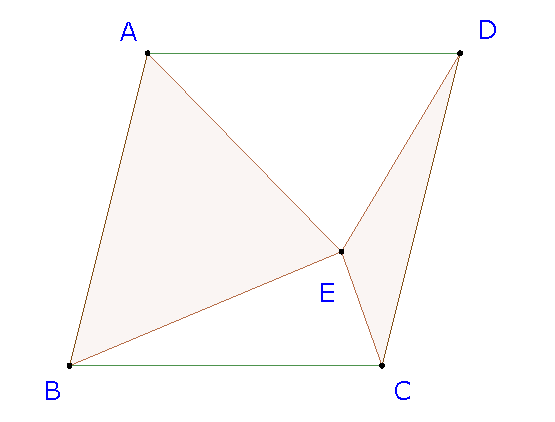
\includegraphics[width= 1\linewidth]{23-24-s3-i-p1.pdf}
		%		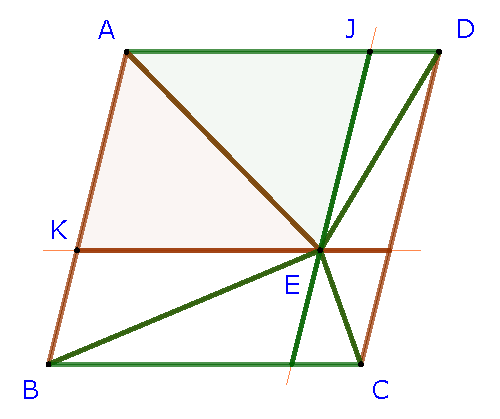
\includegraphics[width= 1\linewidth]{23-24-s3-i-p1-s.pdf}
		\vspace*{-20pt} 
	\end{figure}
	\textit{Solution.}
	Draw lines through $E,$ parallel with sides of $ABCD,$ dividing the parallelogram into four smaller parallelograms.
	Any of the smaller parallelogram, say $AKEJ$, consists of a brown triangle from the shaded triangle and a green triangle with the same area.
	Thus, the area of the shaded triangles is the sum of the area of all smaller brown triangles, which is half of the sum of the area of all smaller parallelograms,
	or half of the $ABCD$ parallelogram.
	\begin{figure}[H]
		%		\vspace*{-10pt}
		\centering
		\captionsetup{labelformat= empty, justification=centering}
		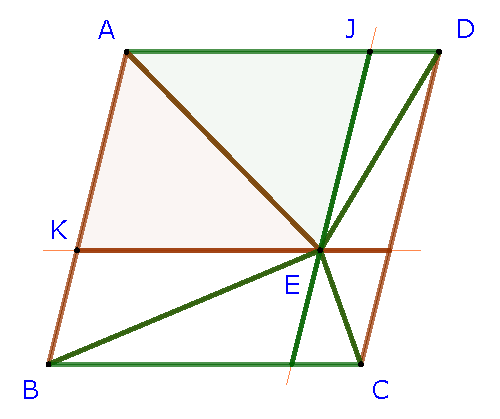
\includegraphics[width= 0.95\linewidth]{23-24-s3-i-p1-s.pdf}
		\vspace*{-10pt} 
	\end{figure}
	\textbf{\color{toancuabi}Remark.} Here's how we use the techniques:
	\vskip 0.1cm
	$1.$ First, divide the given figure into smaller figures.
	\vskip 0.1cm
	$3$. Deal with each of them, if they have the same shape, then work in the same way.
	\vskip 0.1cm
	$3.$ Use all partial results to arrive at the overall result.
	\vskip 0.2cm
	\PIbox{\textbf{\color{toancuabi}Example $\pmb2$.}
		Let $E$ and $F$ be the midpoints of $BC$ and $DA$ in the convex quadrilateral $ABCD$. Prove that
		\begin{align*}
			[AECF] = \half [ABCD].
	\end{align*}}
	\begin{figure}[H]
		\vspace*{-10pt}
		\centering
		\captionsetup{labelformat= empty, justification=centering}
		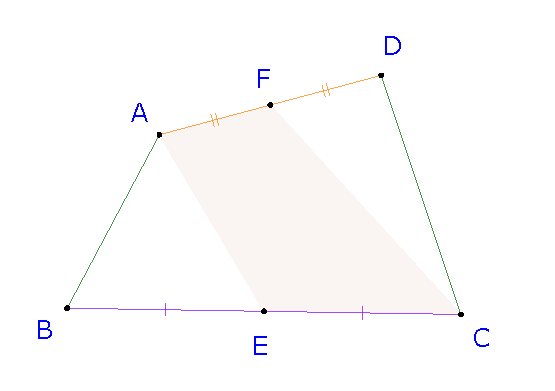
\includegraphics[width= 1\linewidth]{23-24-s3-i-p2.pdf}
		%		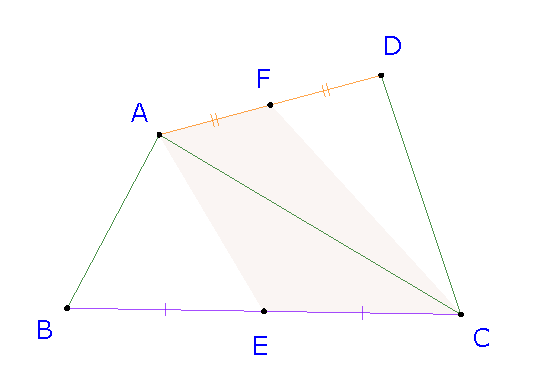
\includegraphics[width= 0.9\linewidth]{23-24-s3-i-p2-s.pdf}
		\vspace*{-20pt}
	\end{figure}
	\textit{Solution.}
	Connect $AC.$ Since $E$ is the midpoint of $BC$, the triangles $ABE$ and $AEC$ have the same area. The triangles $ABE$ and $AEC$ have the same area.
	Similarly triangles $CDF$ and $CFA$ have the same area. Thus the area of $AECF$ is half of $ABCD.$
	\begin{figure}[H]
		\vspace*{-5pt}
		\centering
		\captionsetup{labelformat= empty, justification=centering}
		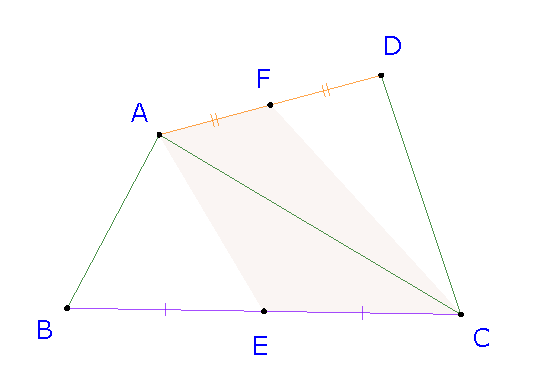
\includegraphics[width= 1\linewidth]{23-24-s3-i-p2-s.pdf}
		\vspace*{-10pt}
	\end{figure}
	\PIbox{\textbf{\color{toancuabi}Example $\pmb3$.}
		Let $I$ be an arbitrary point on the diagonal $BD$ in the parallelogram $ABCD$. Lines through $I$ parallel with the sides of $ABCD$ intersect $AB,$ $BC,$ $CD,$ and $DA$ at $E, F, G,$ and $H,$ respectively. Prove that
		\begin{align*}
			[AEIH] = [FCGI].
	\end{align*}}
	\begin{figure}[H]
		\vspace*{-5pt}
		\centering
		\captionsetup{labelformat= empty, justification=centering}
		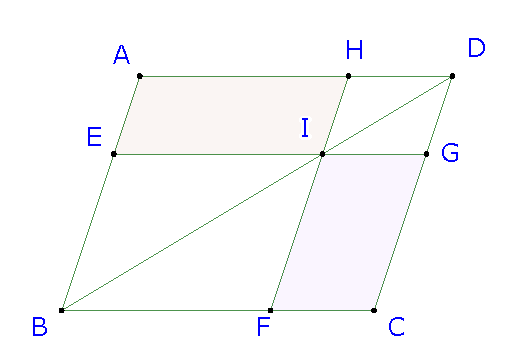
\includegraphics[width= 1\linewidth]{23-24-s3-i-p3.pdf}
		\vspace*{-10pt}
	\end{figure}
	\textit{Solution.}
	First, since $BD$ is the diagonal in parallelogram $ABCD,$ $[ABD] = [BCD].$
	Now, $BEIF$ is also a parallelogram, thus $[BEI] = [BFI],$ similarly $[HID] = [IGD].$
	Therefore 
	\begin{align*}
		[AEIH] &= [ABD] - [BEI] - [HID] \\
		&= [BCD] - [BFI] - [IGD] \\
		&= [FCGI].
	\end{align*}
	\begin{figure}[H]
		\vspace*{-5pt}
		\centering
		\captionsetup{labelformat= empty, justification=centering}
		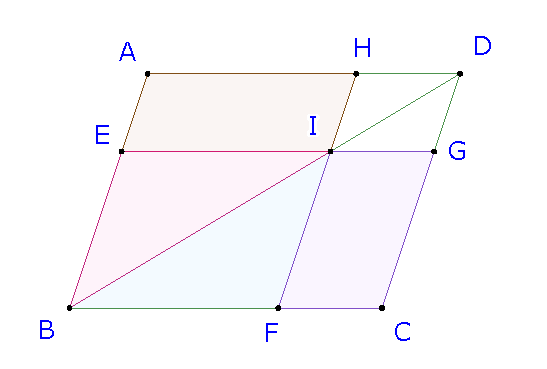
\includegraphics[width= 1\linewidth]{23-24-s3-i-p3-s.pdf}
		\vspace*{-10pt}
	\end{figure}
	\PIbox{\textbf{\color{toancuabi}Example $\pmb4$.} 
		Let $G$ and $H$ be the midpoints of $BC$ and $CD$ in the regular hexagon $ABCDEF$. The lines $EG$ and $FG$ intersect at $I$.  Prove that
		\begin{align*}
			[GCHI] = [EFI].
	\end{align*}}
	\begin{figure}[H]
		\vspace*{-5pt}
		\centering
		\captionsetup{labelformat= empty, justification=centering}
		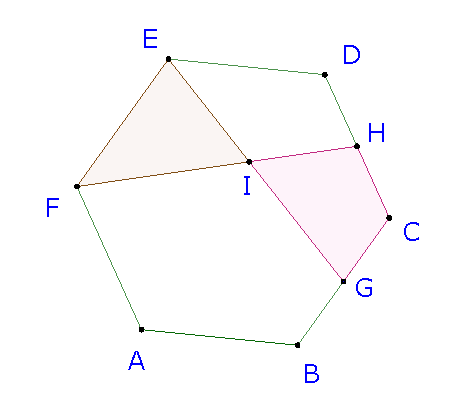
\includegraphics[width= 1\linewidth]{23-24-s3-i-p4.pdf}
		\vspace*{-10pt}
	\end{figure}
	\textit{Solution.}
	It is easy to see that the quadrilaterals $GCDE$ and $HDEF$ are congruent, thus have the same area, or $[GCDE] = [HDEF].$
	Taking $HDEI$ away, we have $[GCHI] = [EFI].$ 
	\vskip 0.2cm
	\PIbox{\textbf{\color{toancuabi}Example $\pmb5$.}
		Let $E, F, G$ and $H$ are the midpoints of the sides $AB, BC, CD$ and $DA$ in the convex quadrilateral $ABCD$.
		Prove that
		\begin{align*}
			[EFGH] = \half [ABCD].
	\end{align*}}
	\begin{figure}[H]
		\vspace*{-5pt}
		\centering
		\captionsetup{labelformat= empty, justification=centering}
		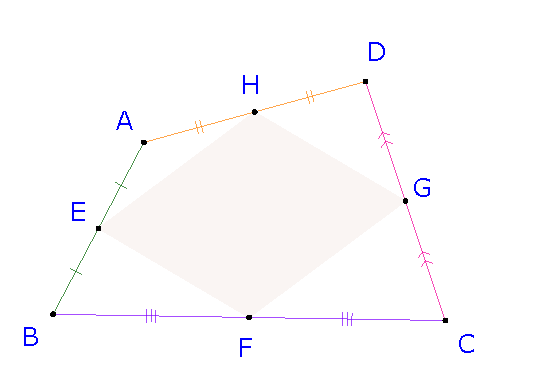
\includegraphics[width= 1\linewidth]{23-24-s3-i-p5.pdf}
		\vspace*{-10pt}
	\end{figure}
	\textit{Solution.}
	Note that $EH$ is the midsegment (the segment joining two midpoints) in the triangle $ABD$, therefore $[AEH] = \frac{1}{4}[ABD].$
	Similarly $[BEF] = \frac{1}{4}[ABC],$ $[CFG] = \frac{1}{4}[BCD],$ and $[GDH] = \frac{1}{4}[CDA],$ therefore:
	\begin{align*}
		&[AEH] + [BEF] + [CFG] + [GDH] \\
		&= \half [ABCD]\\
		\Rightarrow  &[EFGH] = \half [ABCD].
	\end{align*} 
\end{multicols}
\vskip 0.1cm
\PIbox{
	\centerline{\textbf{\color{toancuabi}Vocabulary}}
	\vskip 0.2cm
	\begin{multicols}{2}
		{\color{toancuabi}Arbitrary:} (tt) bất kỳ, tùy ý.
		\vskip 0.1cm	
		{\color{toancuabi}Area:} (dt) diện tích.
		\vskip 0.1cm
		{\color{toancuabi}Congruent:} (tt) bằng nhau.
		\vskip 0.1cm
		{\color{toancuabi}Connect:} (đt) nối.
		\vskip 0.1cm
		{\color{toancuabi}Convex:} (tt) lồi.
		\vskip 0.1cm
		{\color{toancuabi}Diagonal:} (dt) đường chéo
		\vskip 0.1cm
		{\color{toancuabi}Divide:} (đt) chia.
		\vskip 0.1cm
		{\color{toancuabi}Draw:} (đt) kẻ, vẽ.
		\vskip 0.1cm
		{\color{toancuabi}Figure:} (dt) hình.
		\vskip 0.1cm
		{\color{toancuabi}Hexagon:} (dt) lục giác,
		\vskip 0.1cm
		{\color{toancuabi}regular hexagon:} lục giác đều.
		\vskip 0.1cm
		{\color{toancuabi}Intersect:} (đt) cắt nhau, giao nhau.
		\vskip 0.1cm
		{\color{toancuabi}Line:} (dt) đường thẳng.
		\vskip 0.1cm
		{\color{toancuabi}Midpoint:} (dt) trung điểm. 
		\vskip 0.1cm
		{\color{toancuabi}Midsegment:} (dt) đường trung bình.
		\vskip 0.1cm
		{\color{toancuabi}Point:} (dt)  điểm.
		\vskip 0.1cm
		{\color{toancuabi}Parallelogram:} (dt) hình bình hành.
		\vskip 0.1cm
		{\color{toancuabi}Quadrilateral:} (dt)  tứ giác.
		\vskip 0.1cm
		{\color{toancuabi}Segment:} (dt) đoạn thẳng.
		\vskip 0.1cm
		{\color{toancuabi}Shape:} (dt) hình dáng.
		\vskip 0.1cm
		{\color{toancuabi}Side:} (dt) cạnh.
		\vskip 0.1cm
		{\color{toancuabi}Triangle:} (dt)  tam giác.
		\vskip 0.1cm
		{\color{toancuabi}Technique:} (dt) kỹ thuật.
	\end{multicols}
}
